\documentclass[a4paper,10pt]{report}
\usepackage{fullpage}
\usepackage[utf8]{inputenc}
\usepackage[french]{babel}
\usepackage{amsmath}
\usepackage{geometry}
\geometry{hmargin=1.5cm,vmargin=1.5cm}
\usepackage{xcolor}
\usepackage{graphicx}
\usepackage{graphics}
\usepackage{eurosym} %symbole Euro%
\usepackage{color}

\title{Informatique Répartie - Fédération Bancaire}
\date{2015-2016}
\author{Kafui Atanley \\ Quentin Lerebours \\ Florian Leriche \\ Pauline Mouchès}
\begin{document}
\maketitle
\tableofcontents
\chapter{Introduction}

    \include{includes/intro}

%	Dans le cadre du projet d'informatique répartie nous allons concevoir une application répartie permettant la gestion d'une fédération bancaire. Ce présent document de conception a pour objectif de définir l'architecture logicielle de notre application.
%En premier lieu voici les fonctionnalités principales de notre applications :
%	\begin{itemize}
%		\item Un système d'authentification permettant au personnel de se connecter sur l'application.
%		\item La création, consultation et édition des comptes clients.
%		\item La gestion des opérations bancaires telles que les virements, les remises de chèque ainsi que les prêts.
%		\item L'envoi de mail aux clients.
%		\item La gestion de statistiques sur l'ensemble des données.
%		\end{itemize}
%En second lieu, cette application sera proposée à plusieurs type d'utilisateur différents. En effet, elle pourra aussi bien être utilisée par les gérants d'une banque que par les employés. Cependant, les gérants auront tous les droits sur cette application alors que les employés seront gérés par ces derniers. Ces utilisateurs n'étant liés qu'à une banque en particulier, nous avons décidé de mettre en place un troisième type d'utilisateur à savoir gérant de la fédération. \\
%	Pour finir, cette application devra pouvoir fonctionner sous windows et Linux et fonctionnera par le biais d'une architecture client/serveur dans laquelle les clients seront les postes et le serveur sera une unique unité centrale par banque.

\chapter{Specifications}

   \section{Besoins Détaillés}

\subsection{Spécifications Fonctionnelles}

\subsubsection{F1 Utilisateurs}


{\color{orange}{L’application devra permettre de distinguer les différents employés selon le service de la banque auquel ils sont affectés. Il faudra faire attention au fait que cette fédération contient plusieurs banques. Une différentiation au niveau des droits de chaque service devra être faite afin que chaque service puisse échanger des informations avec d’autre service mais garde sa part de confidentialité. Exemple : Le service Ressources Humaines peut envoyer des bilans sur l’effectif total des personnes présentes dans la banque. Le service Ressources Humaines doit pouvoir garder confidentiellement les données concernant le salaire de chaque employé.}}
{\color{green}{L'application permettra de distinguer les employés selon leur rôle: employé, gérant d'une banque ou administrateur de la fédération. Un gérant a la possibilité d'ajouter un nouvel employé ou gérant. L'administrateur de la fédération peut supprimer ou ajouter une banque. La fédération contient plusieurs banques, les
employés et gérants d'une banque ne peuvent pas effectuer d'opération sur les comptes des clients n'appartenant pas à leur banque. Nous avons choisis d'effectuer
cette modification au niveau des rôles pour simplifier l'application. En effet la gestion d'une banque est déjà très complexe, il aurait été difficile pour nous de gérer différents services au sein de chaque banque.}}


\subsubsection{F2 Gestion des comptes client}

Tout les services pourront avoir accès à cette fonctionnalité. Celle-ci devra permettre l’édition de compte à partir desquels nous ferons des virements.Nous pourrons également bloquer et débloquer les comptes. {\color{red}{Cette fonctionnalité permettra également de gérer les prêts des clients, ainsi nous devrons être capable de voir où en est la personne dans ses mensualités, quelle somme il lui reste à rembourser.}} {\color{green}{Nous avons décidé de ne pas gérer les prêts. Nous avons eu un manque de temps et la difficulté de cette fonctionnalité étant semblable à celle des comptes épargne, nous avons jugé peu utile de la créer. Le compte épargne gagne de l'argent tous les mois en fonction d'un taux.}} Il est à noter que la fédération dispose de plusieurs types de compte : compte courant et compte épargne. Il devra également être possible de créer un compte et de le clôturer au moment voulu.

\subsubsection{F3 Envoi de courriels}

Cette fonctionnalité devra permettre l’envoi de courriel au sein de la fédération bancaire.

\subsubsection{F4 Gestion de chèques}

{\color{red}{Cette fonctionnalité devra permettre à chaque service d’effectuer un traitement manuel lors de la réception d’un chèque. La traçabilité est un aspect important de cette fonctionnalité. Ainsi on devra pouvoir savoir de qui vient le chèque et la date à laquelle il a été déposé ainsi que l’employé qui a traité la demande.}}
{\color{green}{Cette fonctionnalité étant similaire à la fonctionnalité permettant de faire de virements, nous avons décidé de ne pas l'implémenter car nous manquions de temps.}}

\subsubsection{F5 Statistiques}

{\color{orange}{Cette fonctionnalité sera accessible à tous les services de chaque banque. Elle devra permettre de suivre le nombre de dépôts de chèques, le nombre de virements à effectuer et la valeur totale du flux monétaire journalier ayant transité.}}
{\color{green}{Nous avons fait des statistiques mais pas celles annoncées, nous avons calculé le nombre de clients de la fédération, le nombre d'opérations effectuées, le nombre de comptes courants et épargnes des banques de la fédération.}}


\subsubsection{F6 Gestion de prêt}

{\color{red}{Cette fonctionnalité devra permettre de mettre à jour en temps réel les différents comptes bancaires vis-à-vis de leurs prêts bancaires.}} {\color{green}{Comme expliqué précédemment, la fonctionnalité de gestion de prêt bancaires n'a pas été implémentée à cause d'un manque de temps et du fait que sa gestion soit similaire à une autre fonctionnalité implémentée}}

\subsection{Constitution des Lots}

\subsubsection{Lot 1}

Ce premier lot à délivrer pour le 21 mars 2016 devra permettre la mise en place de la base de données. La fonctionnalité F1 devra également être terminée.

\subsubsection{Lot 2}

Ce lot à délivrer pour le 11 avril 2016 devra implémenter la fonctionnalité F2 en plus des fonctionnalités développées dans le lot précédent.


\subsubsection{Lot 3}

Ce lot à délivrer pour le 11 mai 2016 devra implémenter les fonctionnalités F3{\color{red}{, F4}}, F5 {\color{red}{et F6}} en plus des fonctionnalités développées dans le lot précédent.

\subsection{Diagramme de Cas d'Utilisation}

\begin{figure}[!h]
\begin{center}

   \caption{\label{} Diagramme de Cas d'Utilisation}
   \includegraphics[scale=0.65]{images/CasUtilisation2.png}
   \centering

\end{center}
\end{figure}

\subsection{Spécifications d'Interface}
La maquette en annexe présente approximativement le résultat visuel que devra fournir l’application.

\subsection{Spécifications Opérationnelles}

\subsubsection{Performances}

L’application devra être performante sous deux systèmes d’exploitation : Linux et Windows. L’application devra supporter d’être utilisée par plusieurs utilisateurs simultanément. {\color{orange}{Ces utilisateurs ne pourront pas accéder au même compte en banque en même temps mais pourront effectuer des manipulations sur des comptes différents en même temps.}}{\color{green}{Les utilisateurs peuvent accéder au même compte en même temps et effectuer des opérations}} Les transactions effectuées sur les comptes tels que par exemple un virement d’argent ou le blocage d’un compte devront avoir un temps de réponse inférieur à une seconde.

\subsubsection{Sécurité, Intégrité et Sûreté}

Tous les utilisateurs de l’application n’auront pas accès à toutes les données. La restriction de leur accès dépendra de leur rôle et de la banque dans laquelle ils travaillent. Les employés d’une banque pourront consulter les comptes et les statistiques des clients d’une autre banque mais ne pourront pas éditer leur compte. Au sein d’une même banque, nous distinguerons deux rôles : les gérants de banque et les employés. Les gérants de banque auront les mêmes accès que les employés et pourront en plus gérer les employés (ajouter {\color{red}{ou supprimer des employés, modifier leur salaire}}).Lors de la connexion, il sera demandé à l’utilisateur d’entrer {\color{orange}{son nom, sa banque et son mot de passe.}} {\color{green}{L'utilisateur a uniquement besoin d'entrer son identifiant et son mot de passe.}} {\color{orange}{Grâce à son nom et sa banque, il sera possible de retrouver son rôle afin d’appliquer les restrictions nécessaires.}}{\color{green}{Grâce à son identifiant, il sera possible de retrouver sa banque et son rôle afin d'appliquer les restrictions nécessaires}}

\subsubsection{Base de Données}

Pour notre projet, nous avons besoin d’une base de données.
Cette base de données stockera tous les noms des clients des différentes banques,
leurs adresses mail afin de pouvoir les avertir automatiquement, l’argent dont ils disposent sur leurs comptes,
{\color{red}{leurs prêts en cours}}{\color{green}{La fonctionnalité de gestion des prêts n'a pas été implémentée}}
et un indicateur permettant de bloquer/débloquer leurs comptes. La base contiendra également le rôle de chaque employé
de chaque banque afin de pouvoir connaître les restrictions à appliquer à son compte. {\color{red}{La base va aussi nous
permettre de stocker différentes données comme par exemple le nombre de virements effectués ou le nombre de chèques
déposés pour pouvoir par la suite réaliser des statistiques.}}
{\color{green}{La base contient la liste des opérations effectuées. À partir de cette liste, il est donc possible de connaître le nombre d'opérations grâce à une simple requête.}}


\section{{\color{orange}{Annexes}}}


{\color{green}{Pour les vues, nous avons remplacé les maquettes par les vues que nous avons réellement créé.}}

\subsection{Vue de connexion}

\begin{figure}[H]
\begin{center}

   \caption{\label{} Formulaire de connexion pour le personnel}
   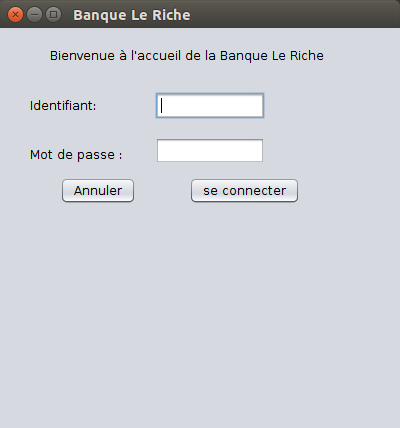
\includegraphics[scale=0.4]{images/connexion.png}
   \centering
 \end{center}
\end{figure}


\subsection{Vues de l'administrateur}

\begin{figure}[H]
\begin{center}

   \caption{\label{} Menu de l'administrateur}
   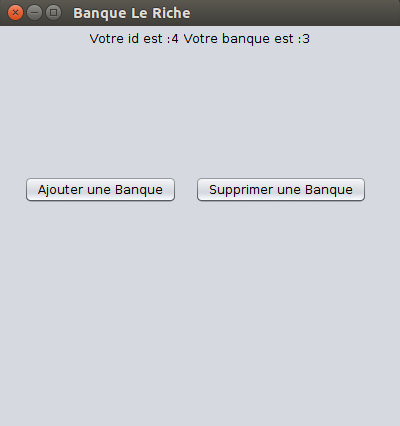
\includegraphics[scale=0.4]{images/adminMenu.png}
   \centering

\end{center}
\end{figure}

\begin{figure}[H]
\begin{center}

   \caption{\label{} Formulaire ajouter banque, disponible uniquement pour l'administrateur}
   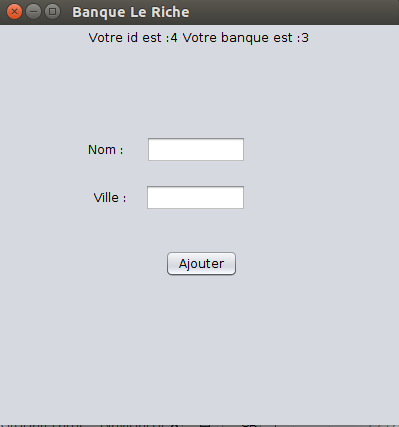
\includegraphics[scale=0.4]{images/AjouterBanque.png}
   \centering
 \end{center}
\end{figure}

 \subsection{Vues de des Gérants et des Employés}

\begin{figure}[H]
\begin{center}

   \caption{\label{} Menu principal}
   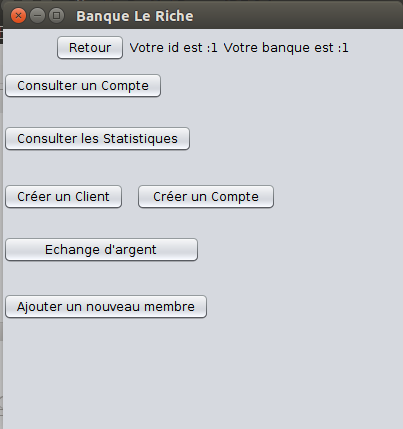
\includegraphics[scale=0.4]{images/gererComptes.png}
   \centering
 \end{center}
\end{figure}

\begin{figure}[H]
\begin{center}

   \caption{\label{} Consulter le ou les comptes d'un client}
   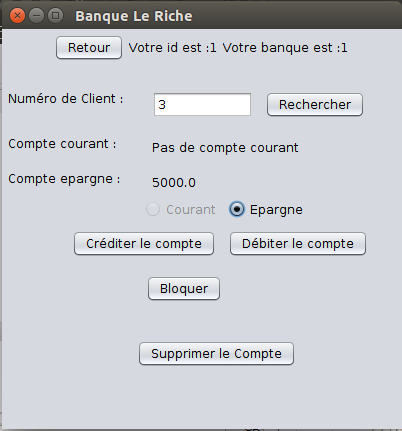
\includegraphics[scale=0.4]{images/ConsulterCompte.png}
   \centering
 \end{center}
\end{figure}

\begin{figure}[H]
\begin{center}

   \caption{\label{} Consulter les statistiques de la fédération}
   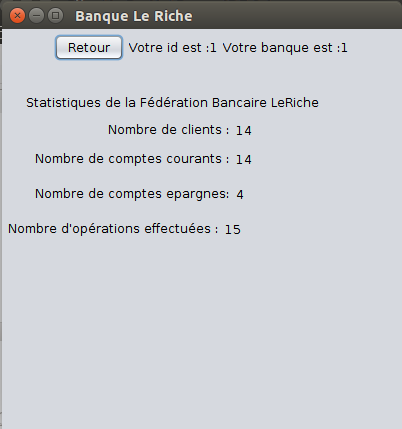
\includegraphics[scale=0.4]{images/Stats.png}
   \centering
 \end{center}
\end{figure}

\begin{figure}[H]
\begin{center}

   \caption{\label{} Formulaire de création d'un client et de son compte}
   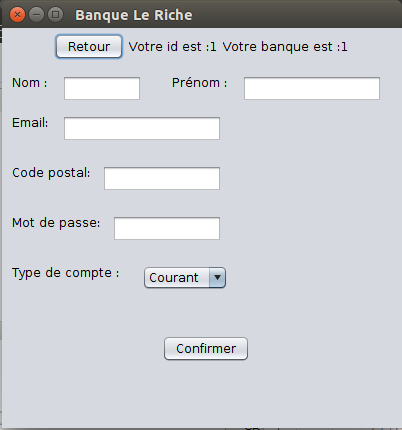
\includegraphics[scale=0.4]{images/creerClient.png}
   \centering
 \end{center}
\end{figure}

\begin{figure}[H]
\begin{center}

   \caption{\label{} Formulaire de création d'un compte associé à un client déjà existant}
   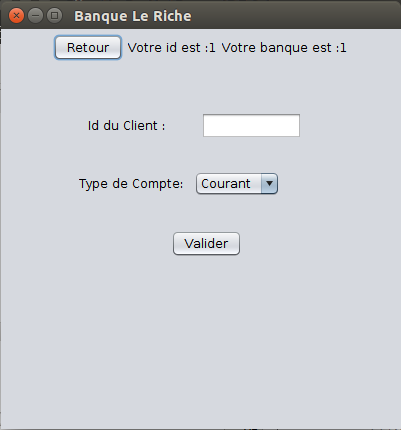
\includegraphics[scale=0.4]{images/CreerCompte.png}
   \centering
 \end{center}
\end{figure}

\begin{figure}[H]
\begin{center}

   \caption{\label{} Effectuer un virement entre deux comptes}
   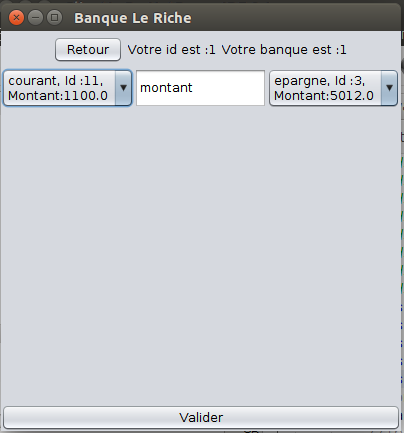
\includegraphics[scale=0.4]{images/EchangeArgent.png}
   \centering
 \end{center}
\end{figure}


\subsection{Vue uniquement visible par les Gérants}

\begin{figure}[H]
\begin{center}

   \caption{\label{} Formulaire de création d'un nouveau membre du personnel}
   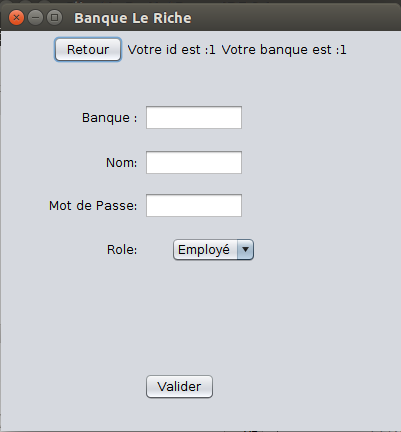
\includegraphics[scale=0.4]{images/CreerPersonnel.png}
   \centering
 \end{center}
\end{figure}



%\section{Besoins Détaillés}
%
%\subsection{Spécifications Fonctionnelles}
%
%\subsubsection{F1 Utilisateurs}
%
%
%{\color{orange}{L’application devra permettre de distinguer les différents employés selon le service de la banque auquel ils sont affectés. Il faudra faire attention au fait que cette fédération contient plusieurs banques. Une différentiation au niveau des droits de chaque service devra être faite afin que chaque service puisse échanger des informations avec d’autre service mais garde sa part de confidentialité. Exemple : Le service Ressources Humaines peut envoyer des bilans sur l’effectif total des personnes présentes dans la banque. Le service Ressources Humaines doit pouvoir garder confidentiellement les données concernant le salaire de chaque employé.}}
%{\color{green}{L'application permettra de distinguer les employés selon leur rôle: employé, gérant d'une banque ou administrateur de la fédération. Un gérant à la possibilité d'ajouter un nouvel employé ou gérant. L'administrateur de la fédération peut supprimer ou ajouter une banque. La fédération contient plusieurs banques, les
%employés et gérants d'une banque ne peuvent pas consulter ni effectuer d'opération sur les comptes des clients n'appartenant pas à leur banque. Nous avons choisis d'effectuer
%cette modification au niveau des rôles pour simplifier l'application. En effet la gestion d'une banque est déjà très complexes, il aurait été difficile pour nous de gérer différents services au sein de chaque banque.}}
%
%
%\subsubsection{F2 Gestion des comptes client}
%
%Tout les services pourront avoir accès à cette fonctionnalité. Celle-ci devra permettre l’édition de compte à partir desquels nous ferons des virements.Nous pourrons également bloquer et débloquer les comptes. {\color{red}{Cette fonctionnalité permettra également de gérer les prêts des clients, ainsi nous devrons être capable de voir où en est la personne dans ses mensualités, quelle somme il lui reste à rembourser.}} {\color{green}{Nous avons décidé de ne pas gérer les prêts. Nous avons eu un manque de temps et la difficulté de cette fonctionnalité étant semblable à celle des comptes épargne, nous avons jugé peu utile de la créer. Le compte épargne gagne de l'argent tous les mois en fonction d'un taux.}} Il est à noter que la fédération dispose de plusieurs types de compte : compte courant et compte épargne. Il devra également être possible de créer un compte et de le clôturer au moment voulu.
%
%\subsubsection{F3 Envoi de courriels}
%
%Cette fonctionnalité devra permettre l’envoi de courriel au sein de la fédération bancaire.
%
%\subsubsection{F4 Gestion de chèques}
%
%{\color{red}{Cette fonctionnalité devra permettre à chaque service d’effectuer un traitement manuel lors de la réception d’un chèque. La traçabilité est un aspect important de cette fonctionnalité. Ainsi on devra pouvoir savoir de qui vient le chèque et la date à laquelle il a été déposé ainsi que l’employé qui a traité la demande.}}
%{\color{green}{Cette fonctionnalité étant similaire à la fonctionnalité permettant de faire de virements, nous avons décidé de ne pas l'implémenter car nous manquions de temps.}}
%
%\subsubsection{F5 Statistiques}
%
%{\color{orange}{Cette fonctionnalité sera accessible à tous les services de chaque banque. Elle devra permettre de suivre le nombre de dépôts de chèques, le nombre de virements à effectuer et la valeur totale du flux monétaire journalier ayant transité.}}
%{\color{green}{Nous avons fait des statistiques mais pas celles annoncées, nous avons calculé le nombre de clients de la fédération, le nombre d'opérations effectuées, le nombre de comptes courants et épargnes des banques de la fédération.}}


%\subsubsection{F6 Gestion de prêt}
%
%{\color{red}{Cette fonctionnalité devra permettre de mettre à jour en temps réel les différents comptes bancaires vis-à-vis de leurs prêts bancaires.}} {\color{green}{Comme expliqué précédemment, la fonctionnalité de gestion de prêt bancaires n'a pas été implémenter à cause d'un manque de temps et du fait que sa gestion soit similaire à une autre fonctionnalité implémentée}}
%
%\subsection{Constitution des lots}
%
%\subsubsection{Lot 1}
%
%Ce premier lot à délivrer pour le 21 mars 2016 devra permettre la mise en place de la base de données. La fonctionnalité F1 devra également être terminée.
%
%\subsubsection{Lot 2}
%
%Ce lot à délivrer pour le 11 avril 2016 devra implémenter la fonctionnalité F2 en plus des fonctionnalités développées dans le lot précédent.
%
%
%\subsubsection{Lot 3}
%
%Ce lot à délivrer pour le 11 mai 2016 devra implémenter les fonctionnalités F3{\color{red}{, F4}}, F5 {\color{red}{et F6}} en plus des fonctionnalités développées dans le lot précédent.
%
%\subsection{Diagramme de cas d'utilisation}
%
%\begin{figure}[!h]
%\begin{center}
%
%   \caption{\label{} Diagramme de Cas d'Utilisation}
%   \includegraphics[scale=0.65]{CasUtilisation2.png}
%   \centering
% 
%\end{center}  
%\end{figure}


\chapter{Conception préliminaire}

    Cette partie contient de nombreux diagrammes permettant de décrire notre application.
\section{Diagramme de modèle du domaine}
\begin{figure}[h!]
\begin{center}
   \caption{\color{orange}{Diagramme de modèle du domaine}}
   \includegraphics[scale=0.5]{images/modeleDuDomaine.png}
   \end{center}
\end{figure}
\newpage
\section{Diagramme d'activité de navigation}
\begin{figure}[h!]
\begin{center}
   \caption{Diagramme de navigation}
   \includegraphics[scale=0.2]{images/navigation.png}
   \end{center}
\end{figure}
\newpage
\section{Diagrammes d'interaction}
\subsection{Cas d'utilisation : Se connecter}
\begin{figure}[h!]
\begin{center}
   \caption{Diagramme d'interaction : Se connecter}
   \includegraphics[scale=0.5]{images/seConnecterIR.png}
   \end{center}
\end{figure}
\subsection{Cas d'utilisation : Créer un compte}
\begin{figure}[h!]
\begin{center}
   \caption{Diagramme d'interaction : Créer un compte}
   \includegraphics[scale=0.4]{images/SInscrire.png}
   \end{center}
\end{figure}
\newpage
\section{{\color{orange}{Diagramme de classes de conception préliminaire}}}
\begin{figure}[h!]
\begin{center}
   \caption{Diagramme de classes}
   \includegraphics[scale=0.4, angle=90]{images/diagrammeClasses.png}
   \end{center}
\end{figure}


%Cette partie contient de nombreux diagrammes permettant de décrire notre application.
%\section{Diagramme de modèle du domaine}
%\begin{figure}[h!]
%\begin{center}
%   \caption{Diagramme de modèle du domaine}
%   \includegraphics[scale=0.5]{modeleDuDomaine.png}
%   \end{center}
%\end{figure}
%\newpage
%\section{Diagramme d'activité de navigation}
%\begin{figure}[h!]
%\begin{center}
%   \caption{Diagramme de navigation}
%   \includegraphics[scale=0.5]{navigation.pdf}
%   \end{center}
%\end{figure}
%\newpage
%\section{Diagrammes d'interaction}
%\subsection{Cas d'utilisation : Se connecter}
%\begin{figure}[h!]
%\begin{center}
%   \caption{Diagramme d'interaction : Se connecter}
%   \includegraphics[scale=0.5]{seConnecterIR.png}
%   \end{center}
%\end{figure}
%\subsection{Cas d'utilisation : Créer un compte}
%\begin{figure}[h!]
%\begin{center}
%   \caption{Diagramme d'interaction : Créer un compte}
%   \includegraphics[scale=0.4]{SInscrire.png}
%   \end{center}
%\end{figure}
%\newpage
%\section{Diagramme de classes de conception préliminaire}
%\begin{figure}[h!]
%\begin{center}
%   \caption{Diagramme de classes}
%   \includegraphics[scale=0.3, angle=90]{diagrammeClasses.png}
%   \end{center}
%\end{figure}
%\newpage


\chapter{Conception détaillée}

    Dans cette partie, chaque package va être décrit. Les attributs et méthodes de chaque classes seront précisées. Le corps des méthodes complexes seront  détaillées grâce à du pseudo-code et commentées.

\section{Package utilisateurs}

\subsection{Banque}

La classe Banque représente une Banque. Une banque possède un nom, une ville et un numéro de banque.
 L'appartenance à une banque des employés permet de définir leur droits sur les comptes bancaires des clients de
 la banque.

\subsection{Personnel}

La classe Personnel représente une personne travaillant dans une des banques de la fédération.
Un personnel possède un nom, un rôle (\color{orange}{Employe, Gerant ou} \color{green}{Admin}),
un identifiant et un mot de passe.
En fonction du rôle et du numéro de banque, on peut déduire les droits du personnel.

\subsection{ClientBanque}

La classe ClientBanque représente un client de la banque possédant un compte Bancaire dans une des banques
de la fédération. Un client de banque possède un nom, un prénom qui permettent d'identifier un et un seul client,
un code postal, un mot de passe, \color{green}{une adresse email} \color{red}{et un numéro de compte} et un numéro de banque.

\section{Package compte}

\subsection{CompteCourant}

La classe CompteCourant représente un compte courant possédé par un client de la banque.
Un compte courant possède un montant, un propriétaire  (un nom et un prénom), un booléen bloqué permettant de bloquer
le compte par exemple en cas de perte de carte bleue, un numéro de compte, un IBAN permettant d'encaisser des chèques
sur le compte.

\subsection{CompteEpargne}

La classe CompteEpargne représente un compte épargne possédé par un client de la banque.
\color{red}{Cette classe hérite de la classe CompteCourant puisque ces deux classes partagent un grand nombre d'attributs. }
\color{green}{Un compte épargne possède les mêmes attributs que le compte courant mais} possède en plus un taux d’intérêt.
Le montant d'un compte épargne augmente chaque année en fonction du taux d’intérêt \color{green}{de façon automatique}.
\color{red}{Sur un compte épargne, il est possible d'effectuer un crédit. Ce crédit sera remboursé chaque mois, en fonction du taux du crédit, grâce à l'argent contenu dans le compte.}

\section{Package transactions}

\subsection{Operation}

La classe Operation représente un opération qui peut un être : créditer ou débiter le compte. Un transaction
possède un montant \color{orange}{(toujours positif), un type (débit ou crédit), un numéro de compte créditeur
et un numéro de compte débiteur}. \color{green}{Une opération entre la banque et un client se symbolisera pas un
virement effectué entre le compte du client et le compte de la banque qui a un numéro précis et fix.}

\subsection{\color{red}{EchangeDArgent}}
\color{red}{La classe EchangeDArgent représente un échange d'argent entre deux comptes via un chèque ou un virement.
Un échange d'argent possède un montant, un numéro de compte de bénéficiaire, un numéro de compte de débiteur et un
type (chèque ou virement).
}

\subsection{\color{red}{Credit}}
\color{red}{La classe Credit représente un crédit, c'est à dire un emprunt réalisé à partir d'un compte épargne.
Un crédit possède un montant, une durée (durée de remboursement), une date d'emprunt et un taux.}

%\section{Package vues}
%
%\subsection{VuePersonnel}
%La classe VuePersonnel représente la vue chargée de fournir une représentation graphique des données concernant le personnel de la banque. Elle devra en outre permettre d'informer le contrôleur dans le cas d'un ajout ou d'une suppression d'un membre du personnel.
%\subsection{VueClientBanque}
%La classe VueClientBanque représente la vue chargée de fournir une représentation graphique des données concernant les clients de la banque. Elle devra en outre permettre d'informer le contrôleur dans le cas d'un ajout d'un client dans la banque.
%
%\subsection{VueCompteCourant}
%La classe VueCompteCourant représente la vue chargée de fournir une représentation graphique des données concernant les comptes courants recensés dans la banque. Elle devra en outre permettre d'informer le contrôleur dans le cas où l'utilisateur souhaite effectuer une opération bancaire.
%
%\subsection{VueCompteEpargne}
%La classe VueCompteEpargne représente la vue chargée de fournir une représentation graphique des données concernant les comptes épargnes recensés dans la banque. Elle devra en outre permettre d'informer le contrôleur dans le cas où l'utilisateur souhaite créer un nouveau crédit.

\section{Package controleur}


\subsection{ControleurClient}
Le contrôleur ControleurClient doit permettre de solliciter le contrôleur serveur afin d'appeler les méthodes adéquates.
Il devra permettre de récupérer les informations dans le but de les empaqueter \color{red}{en RMI}
 \color{green}{en JSON afin de récuperer ces informations en REST}.

\subsection{ControleurServeur}
Le contrôleur ControleurServeur permet d'interpréter les actions de l'utilisateur et d'appeler les méthodes du modèle
dans le but de le mettre à jour. Il permet la gestion des ressources humaines de la banque, des diverses opérations
bancaires ainsi que des comptes bancaires.


%Dans cette partie, chaque package va être décrit. Les attributs et méthodes de chaque classes seront précisées. Le corps des méthodes complexes seront  détaillées grâce à du pseudo-code et commentées.
%
%\section{Package utilisateurs}
%
%\subsection{Banque}
%
%La classe Banque représente une Banque. Une banque possède un nom, une ville et un numéro de banque. L'appartenance à une banque des employés permet de définir leur droits sur les comptes bancaires des clients de la banque.
%
%\subsection{Personnel}
%
%La classe Personnel représente une personne travaillant dans une des banques de la fédération. Un personnel possède un nom, un rôle (employé ou gérant), un identifiant et un mot de passe. En fonction du rôle et du numéro de banque, on peut déduire les droits du personnel.
%
%\subsection{ClientBanque}
%
%La classe ClientBanque représente un client de la banque possédant un compte Bancaire das une des banques de la fédération. Un client de banque possède un nom, un prénom qui permettent d'identifier un et un seul client, un code postal, un mot de passe et un numéro de compte et un numéro de banque.
%
%\section{Package compte}
%
%\subsection{CompteCourant}
%
%La classe CompteCourant représente un compte courant possédé par un client de la banque. Un compte courant possède un montant, un propriétaire  (un nom et un prénom), un booléen bloqué permettant de bloquer le compte par exemple en cas de perte de carte bleue, un numéro de compte, un IBAN permettant d'encaisser des chèques su le compte.
%
%\subsection{CompteEpargne}
%
%La classe CompteEpargne représente un compte épargne possédé par un client de la banque. Cette classe hérite de la classe CompteCourant puisque ces deux classes partagent un grand nombre d'attributs. Un compte épargne possède en plus un taux d’intérêt. Le montant d'un compte épargne augmente chaque année en fonction du taux d’intérêt.  Sur un compte épargne, il est possible d'effectuer un crédit. Ce crédit sera remboursé chaque mois, en fonction du taux du crédit, grâce à l'argent contenu dans le compte.
%
%\section{Package transactions}
%
%\subsection{Operation}
%
%La classe Operation représente un opération qui peut un être : créditer ou débiter le compte. Un transaction possède un montant (positif pour créditer ou négatif pour débiter) et un numéro de compte : le compte sur lequel effectuer la transaction.
%
%\subsection{EchangeDArgent}
%
%La classe EchangeDArgent représente un échange d'argent entre deux comptes via un chèque ou un virement. Un échange d'argent possède un montant, un numéro de compte de bénéficiaire, un numéro de compte de débiteur et un type (chèque ou virement).
%
%\subsection{Credit}
%La classe Credit représente un crédit, c'est à dire un emprunt réalisé à partir d'un compte épargne. Un crédit possède un montant, une durée (durée de remboursement), une date d'emprunt et un taux.
%
%\section{Package vues}
%
%\subsection{VuePersonnel}
%La classe VuePersonnel représente la vue chargée de fournir une représentation graphique des données concernant le personnel de la banque. Elle devra en outre permettre d'informer le contrôleur dans le cas d'un ajout ou d'une suppression d'un membre du personnel.
%\subsection{VueClientBanque}
%La classe VueClientBanque représente la vue chargée de fournir une représentation graphique des données concernant les clients de la banque. Elle devra en outre permettre d'informer le contrôleur dans le cas d'un ajout d'un client dans la banque.
%
%\subsection{VueCompteCourant}
%La classe VueCompteCourant représente la vue chargée de fournir une représentation graphique des données concernant les comptes courants recensés dans la banque. Elle devra en outre permettre d'informer le contrôleur dans le cas où l'utilisateur souhaite effectuer une opération bancaire.
%
%\subsection{VueCompteEpargne}
%La classe VueCompteEpargne représente la vue chargée de fournir une représentation graphique des données concernant les comptes épargnes recensés dans la banque. Elle devra en outre permettre d'informer le contrôleur dans le cas où l'utilisateur souhaite créer un nouveau crédit.
%
%\section{Package controleur}
%
%
%\subsection{ControleurClient}
%Le contrôleur ControleurClient doit permettre de solliciter le contrôleur serveur afin d'appeler les méthodes adéquates. Il devra permettre de récupérer les informations dans le but de les empaqueter en RMI.
%
%\subsection{ControleurServeur}
%Le contrôleur ControleurServeur permet d'interpréter les actions de l'utilisateur et d'appeler les méthodes du modèle dans le but de le mettre à jour. Il permet la gestion des ressources humaines de la banque, des diverses opérations bancaires ainsi que des comptes bancaires.
%détail des méthodes

\chapter{Implémentation et tests}
    \newpage
\section{Application Serveur}
\subsection{Description}
Pour commencer, nous avons décidé de mettre en place une architecture REST pour notre application. La contrainte client serveur nous a imposé
une séparation des responsabilités entre le serveur d'application et les divers clients. 
Nous avons décidé d'utiliser resteasy, un projet JBOSS fournissant un framework dans le but de concevoir des applications java RESTful et des web services RESTful.\\
Il s'agit d'une implémentation de la spécification JAX-RS utilisant le protocol HTTP.
Ensuite, dans le but de stocker nos données nous avons choisi de mettre en place une base de données gérer via le sgbd MySQL. De plus, afin de rester concentré
sur un paradigme de programmation objet, nous avons décidé d'avoir recours à l'ORM Hibernate. 
\\
Hibernate est un framework open source qui permet de gérer la persistance des objets en base de données relationnelle.
Son principal avantage est de masquer la logique relationnelle aux développeurs et de leur permettre de se concentrer
sur un seul paradigme de programmation, à savoir objet. En effet, ce dernier permet de représenter les tables de la base 
de données en objet. De plus, il est plus facile pour une application java de manipuler des objets java que d'utiliser des drivers dans le but d'accéder aux champs de la base de données. Ensuite, Hibernate est une surcouche qui a un un coût en ressource.
Cependant il offre une bonne gestion de cache qui permet un gain en performance. Enfin, ce dernier possède un système de session assurant l'unicité et la cohérence des objets, accompagné d'un système transactionnel.
\\
La création de l'interface homme machine de notre application ayant été déléguée, nous avons décidé de créer un client de test dans un terminal, dépourvu de toute interface visuelle dans l'optique de tester nos requêtes et nos méthodes créés côté serveur en totale indépendance avec le client.




\newpage
\section{Application Cliente}
\subsection{Description}

Au début du projet nous avions pour idée d'effectuer une application cliente comprenant uniquement quatre vues. 
Nous étions dans l'optique d'appliquer le patron de conception "Modèle-Vue-Contrôleur".
Nous avons finalement jugé plus intéressant de détacher les vues des entités nécessaires côté serveur afin de permettre un potentiel développement d'un client dans un autre langage. \\
Comme visible sur le diagramme de classe il y a un package "Metier".
Celui-ci permet d'établir la connexion avec l'application serveur.\\
Il y a également un package "Security" utilisé par le package "Metier", il permet le cryptage/décryptage des données envoyées/reçues.
Ce package sera détaillé ultérieurement dans la partie **faire un lien**.
Dans le cadre de ce projet nous n'avons pas renforcé la vérification côté client car nous voulions investir un maximum de temps sur la partie distribution de la technologie.

\subsection{Interface Graphique}

Pour réaliser notre application, nous avons décidé d'utiliser la bibliothèque graphique Swing proposée par Java. Nous avons créé une JFrame qui contient un JPanel dont le Layout est CardLayout. Il est possible d'ajouter de nombreux composants à un CardLayout et de les rendre visible lorsqu'on le souhaite.
 Nous avons créé un JPanel par vue et nous avons ajouté tous les JPanel au CradLayout. Il nous est ainsi très simple de passer d'un JPanel à un autre lors d'un événement comme par exemple lors de l'appui sur un bouton. \\
Les vues permettent à l'utilisateur de visualiser les données mais aussi de modifier les données en éditant ou créant des comptes par exemple. Nous avons ajouté un grand nombre de pop-ups à notre application afin d'avertir l'utilisateur lorsqu'il entre des données erronées mais aussi afin de réduire le nombre de vues. En effet l'action créditer un compte, par exemple, ne possède pas de vue.\\ 
Lorsque l'utilisateur veut créditer un compte, un pop-up s'ouvre afin de lui demander le montant. Les vues interagissent avec les classes de package "Metier" décrit ci-dessous. Elles appellent les méthodes contenues dans ce package et permettent à l'utilisateur d'obtenir un affichage simple et compréhensible des données.


\subsection{Partie métier}
Ce package permet de faire la jonction entre l'application cliente et l'application serveur. 
En effet à partir des données récupérées via l'interface graphique, c'est ce package qui permet de faire les requêtes nécessaires au serveur. Ce package permet ensuite de faire suivre les réponses du serveur aux classes du package de l'interface graphique qui les met en forme.
Chaque classe graphique ayant besoin de requêtes qui lui sont spécifiques, nous avons décidé de nommer chaque classe par le même nom que son correspondant graphique en lui ajoutant le suffixe R. \\
Les requêtes ont été effectué grâce à la librairie Java RestEasy.
Ce package est dépendant du package sécurité car les données se doivent d'être envoyées chiffrées pour pouvoir être interprétées par le serveur.\\


\newpage
\section{Sécurité}

\subsection{Description}
Afin d'assurer la sécurité de notre application nous avons décidé de mettre en place un cryptage des flux entre l'application cliente et l'application serveur.
L’identifiant des ressources est également chiffré, empêchant ainsi à une personne quelconque de consulter une ressource.
En somme deux algorithmes de cryptage sont utilisées : 
\begin{itemize}
\item Un algorithme pour crypter les données.
\item Un algorithme pour crypter les identifiants de ressources.
\end{itemize}
Cet algorithme de cryptage nous permet d'envoyer les données avec pour en-tête "text/plain". 
En effet seul nous (concepteurs de l'application) savons que les ressources envoyées sont sous format json. Envoyer les données avec pour en-tête "application/xml" donnerait des indications sur le contenu de la donnée à un potentiel attaquant.
Si jamais une personne venait à découvrir l'algorithme de cryptage des identifiants de ressource, il faudrait encore qu'elle brise l'algorithme de cryptage des données.

\subsection{Cryptage des données}
Pour assurer le cryptage des données nous avons utilisé l'algorithme de cryptage AES. Nous avons choisi d'utiliser celui-ci car il est très connu pour sa robustesse et sa grande utilisation fait objet d'une documentation approfondie nous ayant permis de le prendre en main assez rapidement.
Si jamais une personne venait à découvrir l'algorithme utilisé pour chiffrer les données, encore faudrait-il qu'elle découvre la clef de chiffrement pour pouvoir décrypter les données.

Difficultés rencontrées : \\
Lorsque nous avons commencé à crypter les données, nous utilisions le même algorithme pour chiffrer les identifiants de ressources et les données qu'elles contenaient.
Nous avons alors rencontré des problèmes car avec la clef de chiffrage choisie l'identifiant "5" était traduit par une expression de type "aza/4qd/ddqe\&".
Dû à la présence du caractère "/", le serveur cherchait à parser vers une ressource qui n'en était pas une.\\
C'est dans ce contexte que nous avons décidé de mettre en place notre propre algorithme de cryptage d'identifiant de ressource.

\subsection{Cryptage des identifiants}

Nous avons mis en place notre propre algorithme de cryptage d'identifiant mais nous aurions très bien pu utiliser un algorithme de cryptage n'utilisant pas le caractère spécial "/".\\
C'est un algorithme de cryptage qui prend un identifiant "entier", le transforme mathématiquement et ajoute un chiffre permettant de connaître la parité de l'identifiant initialement envoyé.
Le serveur dispose uniquement de la méthode pour décrypter l'identifiant là où le client dispose uniquement de la méthode pour crypter l'identifiant.

\newpage
\section{Test}

Cette partie fait état des différents tests de validation effectués.
Attention : Les flux de données étant chiffrés, la volonté de vouloir tester l'application serveur indépendamment de l'application cliente nécessite d'utiliser la classe Encrypt.\\
Les URL données ci-dessous sont à préfixer de l'adresse de déploiement.

\subsection{Test 1 : S'identifier}

Ce test permet de vérifier que la connexion au serveur est fonctionnelle.
Celle-ci s'effectue via une requête de type GET à l'URL suivante "/personnel/{id}".
La vérification du mot de passe s'effectue côté client. 
\\
L'application cliente développée permet une utilisation facilitée de cette fonctionnalité. 
\\
\textbf{\underline{Réussite}} : Le serveur renvoie un status 200 de la requête HTTP et récupère le fichier JSON chiffré. Ce test peut s'effectuer via l'interface graphique en essayant de se connecter via l'accueil.\\
\\
\textbf{\underline{Échec}} : Le serveur renvoie un status 200 mais les données JSON récupérées signalent un échec de la transaction reçue.
L'application cliente permet de récupérer le mot de passe à partir de la ressource reçue. Si le mot de passe ne concorde pas ou si la ressource demandée n'existe pas, une fenêtre apparaît pour détailler le problème.

\subsection{Test 2 : Créer un client}

Ce test permet de vérifier que la création d'un client est fonctionnelle.
Celle-ci s'effectue via une requête de type POST à l'URL suivante "/client/creer" .
\\
L'application cliente développée permet une utilisation facilitée de cette fonctionnalité. 
\\
\textbf{\underline{Réussite}} : Le serveur renvoie un status de type 200 ainsi que les données chiffrées concernant le nouveau client. Un nouveau client est entré dans la base de données.
L'application cliente développée dispose d'un bouton pour tout personnel faisant parti de la catégorie Gérant/Employé permettant de créer un client conjointement avec son compte épargne/courant.
\\
\textbf{\underline{Échec}} : Le serveur renvoie un status de type 500.

\subsection{Test 3 : Consulter un compte}

Ce test permet de vérifier que la consultation d'un compte est fonctionnelle.
Celle-ci s'effectue via une requête de type GET aux URLs suivantes "/compte/courant/{id}" et "/compte/epargne/{id}" .
L'identifiant de la ressource du compte est chiffrée.
\\
L'application cliente développée permet une utilisation facilitée de cette fonctionnalité. 
\\
\textbf{\underline{Réussite}} : Le serveur renvoie un status de type 200 ainsi que les données chiffrées concernant le compte en question.
L'application cliente développée dispose d'un bouton pour tout personnel faisant partie de la catégorie Admin/Employé permettant de consulter un compte.
\\
\textbf{\underline{Échec}} : Le serveur renvoie un status de type 500.

\subsection{Test 4 : Échange d'argent}

Ce test permet de vérifier que le transfert d'argent d'un compte à un autre est fonctionnelle.
Celui-ci s'effectue via une requête de type POST à l’URL suivante "/client/compte/operer".
\\
L'application cliente développée permet une utilisation facilitée de cette fonctionnalité. 
\\
\textbf{\underline{Réussite}} :Le serveur renvoie un status de type 200 ainsi que les données chiffrées concernant les comptes en questions.
L'application cliente développée dispose d'un bouton pour tout personnel faisant partie de la catégorie Admin/Employé permettant d'échanger de l'argent.
\\
\textbf{\underline{Échec}} : Le serveur renvoie un status de type 500.

\subsection{Test 5 : Bloquer un compte}

Ce test permet de vérifier que le blocage d'un compte est fonctionnelle.
Celui-ci s'effectue via une requête de type PUT à l’URL suivante "/client/compte/bloquer".
\\
L'application cliente développée permet une utilisation facilitée de cette fonctionnalité. 
\\
\textbf{\underline{Réussite}} : Le serveur renvoie un status de type 200 ainsi que les données chiffrées concernant les comptes en questions.
Il faut se connecter en ayant un compte de type employé/gérant. Il faut ensuite cliquer sur consulter un compte. Après avoir rentré un id client, l'option "bloquer un compte" est proposée.
\\
\textbf{\underline{Échec}} :  Le serveur renvoie un status de type 500.

\subsection{Test 6 : Ajouter un nouveau membre}

Ce test permet de vérifier que l'ajout d'un membre du personnel est fonctionnelle.
Celle-ci s'effectue via une requête de type POST à l'URL suivante "/personnel/creer" .
\\
L'application cliente développée permet une utilisation facilitée de cette fonctionnalité. 
\\
\textbf{\underline{Réussite}} : Le serveur renvoie un status de type 200 ainsi que les données chiffrées concernant le nouveau client. Un nouveau membre du personnel est ajouté dans la base de données.
L'application cliente développée dispose d'un bouton pour tout personnel faisant parti de la catégorie Admin/Employé permettant d'ajouter un membre du personnel.
Attention : Le champs banque attends l'id de la banque auquel le nouveau membre sera ajouté.
\\
\textbf{\underline{Échec}} : Le serveur renvoie un status de type 500.

\subsection{Test 7 : Consulter les Statistiques}
Ce test permet de vérifier que la consultation de statistiques est fonctionnelle .
Celle-ci s'effectue via grâce des requêtes de types GET aux URL suivantes "/stats/clients","/stats/operations","/stats/comptes" .

L'application cliente développée permet une utilisation facilitée de cette fonctionnalité. 
Elle dispose d'un bouton pour tout personnel faisant partie de la catégorie Admin/Employé permettant de consulter les statistiques de sa banque.
\\
\textbf{\underline{Réussite}} : Le serveur renvoie un status de type 200 ainsi que les données chiffrées concernant les statistiques.
L'application cliente développée dispose d'un bouton pour tout personnel faisant partie de la catégorie Admin/Employé permettant d'ajouter un membre du personnel.
\\
\textbf{\underline{Échec}} : Le serveur renvoie un status de type 500.

\subsection{Test 8 : Créer un compte }

Ce test permet de vérifier que l'ajout d'un compte à un client existant est fonctionnelle .
Celle-ci s'effectue grâce des requêtes de types GET aux URL suivantes "/client/compte-courant",/client/compte-epargne" .

L'application cliente développée permet une utilisation facilitée de cette fonctionnalité. 

\textbf{\underline{Réussite}} : Le serveur renvoie un status de type 200 ainsi que les données chiffrées concernant le client concerné. Un nouveau compte est entré dans la base de données.
L'application cliente développée dispose d'un bouton pour tout personnel faisant parti de la catégorie Admin/Employé permettant de créer un compte.
Attention : Il faut rentrer l'id du client.
\\
\textbf{\underline{Échec}} : Le serveur renvoie un status de type 500.

\subsection{Test 9 : Créditer/Débiter le compte}

Ce test permet de vérifier que le débit/crédit d'un compte existant est fonctionnelle .
Celui-ci s'effectue grâce à une requête de type POST à l'URL suivante "/client/compte/operer" .

L'application cliente développée permet une utilisation facilitée de cette fonctionnalité. 

\textbf{\underline{Réussite}} : Le serveur renvoie un status de type 200.
L'application cliente développée dispose d'un bouton pour tout personnel faisant parti de la catégorie Admin/Employé permettant de consulter les comptes des clients.
L'interface propose ensuite de créditer/débiter un compte.
\\
\textbf{\underline{Échec}} : Le serveur renvoie un status de type 500.

\subsection{Test 10 : Ajouter une banque}

Le test permet de vérifier que l'ajout d'une banque est fonctionnelle .
Celle-ci s'effectue via grâce à une requête de type POST à l'URL suivante "/creer" .

\textbf{\underline{Réussite}} : Le serveur renvoie un status de type 200 ainsi que les données chiffrées concernant la banque créé. Une nouvelle banque est entrée dans la base de données.
L'application cliente développée dispose d'un bouton pour tout personnel faisant parti de la catégorie Admin permettant de créer une banque.
Attention : Il faut rentrer l'id du client.
\\
\textbf{\underline{Échec}} : Le serveur renvoie un status de type 500.


\subsection{Test 11 : Supprimer une banque}

Le test permet de vérifier que l'ajout d'une banque est fonctionnelle .
Celle-ci s'effectue via grâce à une requête de type DELETE à l'URL suivante "/supprimer/{id}" .

\textbf{\underline{Réussite}} : Le serveur renvoie un status de type 200.
L'application cliente développée dispose d'un bouton pour tout personnel faisant partie de la catégorie Admin permettant de supprimer une banque. La banque est supprimée de la base de données.
\\
\textbf{\underline{Échec}} : Le serveur renvoie un status de type 500.

\subsection{Test 12 : Gestion des accès concurrents}

Le test permet de vérifier que les accès concurents à la base de données sont fonctionnelles .
Celle-ci s'effectue via l'interface graphique en essayant de supprimer un client.
Pour cela il faut ouvrir deux applications clientes et essayer de supprimer un même compte.

\textbf{\underline{Réussite}} : Les données sont bien mises à jour dans l'ordre dans la base de données.
\\
\textbf{\underline{Échec}} : Le serveur renvoie un status de type 500.

\subsection{Test 13 : Portabilité de l'application}

Tous les tests décrits antérieurement ont été exécutés sur Linux et sur Windows 10.



\chapter{Conclusion et perspectives}
    \include{includes/conclu}

\end{document}\grid
\grid
